\section{Motor Back EMF}

After the compensation steps outlined in section \ref{sec:basic}, the amplifier behaves more or less linearly given a resistive load.
The nonlinearity and difference from simulated curve in figure \ref{fig:ioactual} is caused primarily by motor back EMF.
A PWM amplifier, the type of amplifier being used here, is essentially an open-loop power amplifier that allows current to pass for a certain fraction of each oscillation period. 
It does not inherently control voltage and the voltage seen at the amplifier terminals depends on the characteristics of the load.

It is possible to account for back EMF given that the speed of the motor is known by way of encoder feedback.
A simple compensation block diagram to account for back EMF is shown in figure \ref{fig:iobackemfcomp}.
The actual simulink block used, including both basic and back EMF compensation, may be seen in figure \ref{fig:simulink}.
Due to the dependence on having an actual motor to test, no data has been collected to test the back EMF compensator.
The gain shown in figure \ref{fig:iobackemfcomp} is the motors $K_b$ parameter assuming speed is measured in radians per second.

\begin{figure}[ht]
    \centering
    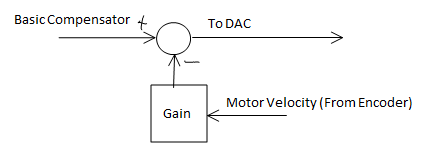
\includegraphics[width=.35\textwidth]{images/BackEMFCompensator.PNG}
    \caption{Back EMF Compensation Block Diagram}
    \label{fig:iobackemfcomp}
\end{figure}

